\documentclass[12pt, a4paper, oneside]{article}\usepackage[]{graphicx}\usepackage[]{color}
%% maxwidth is the original width if it is less than linewidth
%% otherwise use linewidth (to make sure the graphics do not exceed the margin)
\makeatletter
\def\maxwidth{ %
  \ifdim\Gin@nat@width>\linewidth
    \linewidth
  \else
    \Gin@nat@width
  \fi
}
\makeatother

\definecolor{fgcolor}{rgb}{0.345, 0.345, 0.345}
\newcommand{\hlnum}[1]{\textcolor[rgb]{0.686,0.059,0.569}{#1}}%
\newcommand{\hlstr}[1]{\textcolor[rgb]{0.192,0.494,0.8}{#1}}%
\newcommand{\hlcom}[1]{\textcolor[rgb]{0.678,0.584,0.686}{\textit{#1}}}%
\newcommand{\hlopt}[1]{\textcolor[rgb]{0,0,0}{#1}}%
\newcommand{\hlstd}[1]{\textcolor[rgb]{0.345,0.345,0.345}{#1}}%
\newcommand{\hlkwa}[1]{\textcolor[rgb]{0.161,0.373,0.58}{\textbf{#1}}}%
\newcommand{\hlkwb}[1]{\textcolor[rgb]{0.69,0.353,0.396}{#1}}%
\newcommand{\hlkwc}[1]{\textcolor[rgb]{0.333,0.667,0.333}{#1}}%
\newcommand{\hlkwd}[1]{\textcolor[rgb]{0.737,0.353,0.396}{\textbf{#1}}}%

\usepackage{framed}
\makeatletter
\newenvironment{kframe}{%
 \def\at@end@of@kframe{}%
 \ifinner\ifhmode%
  \def\at@end@of@kframe{\end{minipage}}%
  \begin{minipage}{\columnwidth}%
 \fi\fi%
 \def\FrameCommand##1{\hskip\@totalleftmargin \hskip-\fboxsep
 \colorbox{shadecolor}{##1}\hskip-\fboxsep
     % There is no \\@totalrightmargin, so:
     \hskip-\linewidth \hskip-\@totalleftmargin \hskip\columnwidth}%
 \MakeFramed {\advance\hsize-\width
   \@totalleftmargin\z@ \linewidth\hsize
   \@setminipage}}%
 {\par\unskip\endMakeFramed%
 \at@end@of@kframe}
\makeatother

\definecolor{shadecolor}{rgb}{.97, .97, .97}
\definecolor{messagecolor}{rgb}{0, 0, 0}
\definecolor{warningcolor}{rgb}{1, 0, 1}
\definecolor{errorcolor}{rgb}{1, 0, 0}
\newenvironment{knitrout}{}{} % an empty environment to be redefined in TeX

\usepackage{alltt} % Paper size, default font size and one-sided paper
%\graphicspath{{./Figures/}} % Specifies the directory where pictures are stored
%\usepackage[dcucite]{harvard}
\usepackage{amsmath}
\usepackage{setspace}
\usepackage{pdflscape}
\usepackage{rotating}
\usepackage[flushleft]{threeparttable}
\usepackage{multirow}
\usepackage[comma, sort&compress]{natbib}% Use the natbib reference package - read up on this to edit the reference style; if you want text (e.g. Smith et al., 2012) for the in-text references (instead of numbers), remove 'numbers' 
\usepackage{graphicx}
%\bibliographystyle{plainnat}
\bibliographystyle{agsm}
\usepackage[colorlinks = true, citecolor = blue, linkcolor = blue]{hyperref}
%\hypersetup{urlcolor=blue, colorlinks=true} % Colors hyperlinks in blue - change to black if annoying
%\renewcommand[\harvardurl]{URL: \url}
\IfFileExists{upquote.sty}{\usepackage{upquote}}{}
\begin{document}
\title{Yield Curve Modeling}
\author{Rob Hayward}
\date{\today}
\maketitle
This comes from \href{http://blog.revolutionanalytics.com/2014/07/quantitative-finance-applications-in-r-7-constructing-a-term-structure-of-interest-rates-using-r-par.html}{Yield Curve Modeling}

This based on the simple model that the return to a security evolves acording to the mechanics of \emph{Brownian motion}

\begin{equation}
\mu \Delta t + \sigma Z \sqrt{\delta t}
\end{equation}

Where $\mu$ is the mean annual return of the security (also called the drift), $\sigma$ is the annualised volatility (standard deviation), Z is a standard Normal random variable which introduces the stochastic element. Time is measured in units of years (t).  Therefore a quarter is $t/4$.  

To generate a simulated distribution of quarterly returns when $\mu = 10\%$ and $\sigma = 15\%$ 

\begin{knitrout}
\definecolor{shadecolor}{rgb}{0.969, 0.969, 0.969}\color{fgcolor}\begin{kframe}
\begin{alltt}
\hlstd{n} \hlkwb{<-} \hlnum{10000}
\hlkwd{set.seed}\hlstd{(}\hlnum{106}\hlstd{)}
\hlstd{z} \hlkwb{<-} \hlkwd{rnorm}\hlstd{(n)}
\hlstd{mu} \hlkwb{<-} \hlnum{0.1}
\hlstd{sd} \hlkwb{<-} \hlnum{0.15}
\hlstd{delta_t} \hlkwb{<-} \hlnum{0.25}
\hlstd{qrt_returns} \hlkwb{<-} \hlstd{mu} \hlopt{*} \hlstd{delta_t} \hlopt{+} \hlstd{sd} \hlopt{*} \hlstd{z} \hlopt{*} \hlkwd{sqrt}\hlstd{(delta_t)}
\hlkwd{hist}\hlstd{(qrt_returns,} \hlkwc{breaks} \hlstd{=} \hlnum{100}\hlstd{,} \hlkwc{col} \hlstd{=} \hlstr{"green"}\hlstd{)}
\end{alltt}
\end{kframe}
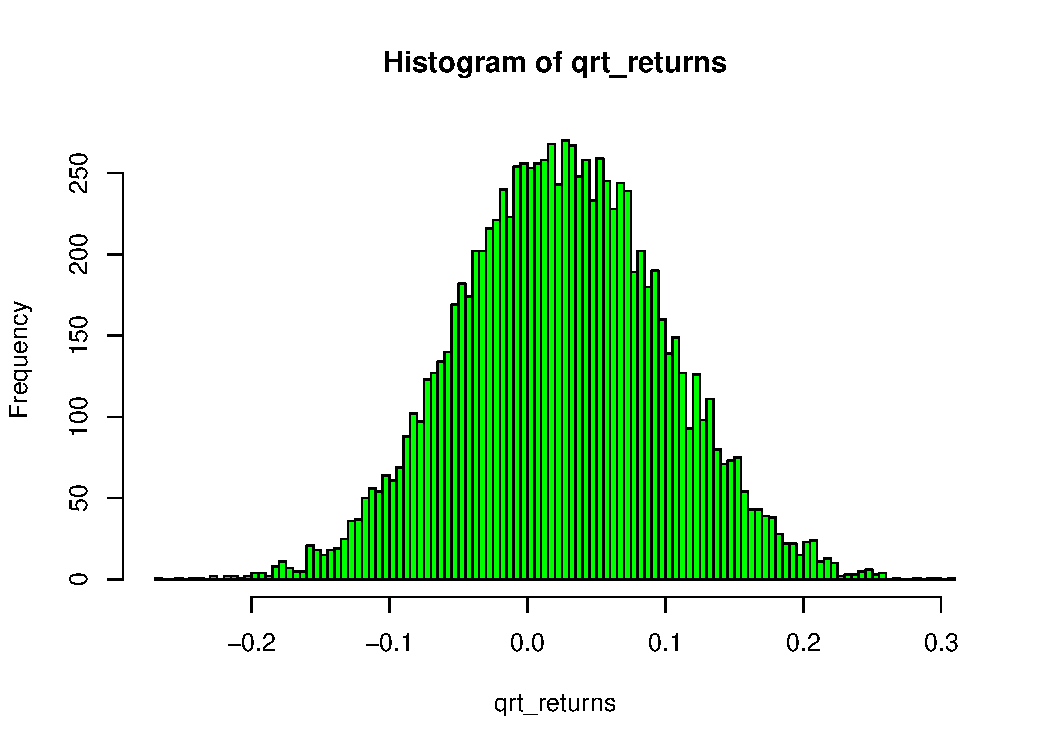
\includegraphics[width=\maxwidth]{figure/returns} 
\begin{kframe}\begin{alltt}
\hlstd{stats} \hlkwb{<-} \hlkwd{c}\hlstd{(}\hlkwd{mean}\hlstd{(qrt_returns)} \hlopt{*} \hlnum{4}\hlstd{,} \hlkwd{sd}\hlstd{(qrt_returns)} \hlopt{*} \hlnum{2}\hlstd{)}
\hlkwd{names}\hlstd{(stats)} \hlkwb{<-} \hlkwd{c}\hlstd{(}\hlstr{"mean"}\hlstd{,} \hlstr{"volatility"}\hlstd{)}
\hlstd{stats}
\end{alltt}
\begin{verbatim}
##       mean volatility 
##    0.09901    0.14976
\end{verbatim}
\end{kframe}
\end{knitrout}

This is close to the assumption that the return was 10\% and the volatility 15\%. 
Now it is necessary to take the dates for the yeild curve. 

\begin{knitrout}
\definecolor{shadecolor}{rgb}{0.969, 0.969, 0.969}\color{fgcolor}\begin{kframe}
\begin{alltt}
\hlkwd{require}\hlstd{(lubridate)}
\hlkwd{require}\hlstd{(xts)}
\hlkwd{require}\hlstd{(lubridate)}
\hlkwd{require}\hlstd{(xts)}
\hlstd{ad} \hlkwb{<-} \hlkwd{ymd}\hlstd{(}\hlnum{20140514}\hlstd{,} \hlkwc{tz} \hlstd{=} \hlstr{"UTC"}\hlstd{)}
\hlstd{marketDates} \hlkwb{<-} \hlkwd{c}\hlstd{(ad, ad} \hlopt{+} \hlkwd{days}\hlstd{(}\hlnum{1}\hlstd{), ad} \hlopt{+} \hlkwd{weeks}\hlstd{(}\hlnum{1}\hlstd{), ad} \hlopt{+} \hlkwd{months}\hlstd{(}\hlnum{1}\hlstd{), ad} \hlopt{+} \hlkwd{months}\hlstd{(}\hlnum{2}\hlstd{),}
    \hlstd{ad} \hlopt{+} \hlkwd{months}\hlstd{(}\hlnum{3}\hlstd{), ad} \hlopt{+} \hlkwd{months}\hlstd{(}\hlnum{6}\hlstd{), ad} \hlopt{+} \hlkwd{months}\hlstd{(}\hlnum{9}\hlstd{), ad} \hlopt{+} \hlkwd{years}\hlstd{(}\hlnum{1}\hlstd{),} \hlkwc{ad} \hlstd{=} \hlkwd{years}\hlstd{(}\hlnum{2}\hlstd{),}
    \hlstd{ad} \hlopt{+} \hlkwd{years}\hlstd{(}\hlnum{3}\hlstd{), ad} \hlopt{+} \hlkwd{years}\hlstd{(}\hlnum{5}\hlstd{), ad} \hlopt{+} \hlkwd{years}\hlstd{(}\hlnum{7}\hlstd{), ad} \hlopt{+} \hlkwd{years}\hlstd{(}\hlnum{10}\hlstd{), ad} \hlopt{+} \hlkwd{years}\hlstd{(}\hlnum{15}\hlstd{),}
    \hlstd{ad} \hlopt{+} \hlkwd{years}\hlstd{(}\hlnum{20}\hlstd{), ad} \hlopt{+} \hlkwd{years}\hlstd{(}\hlnum{25}\hlstd{), ad} \hlopt{+} \hlkwd{years}\hlstd{(}\hlnum{30}\hlstd{))}
\hlcom{# use substring() to get rid of the time zone.}
\hlstd{marketDates} \hlkwb{<-} \hlkwd{as.Date}\hlstd{(}\hlkwd{substring}\hlstd{(marketDates,} \hlnum{1}\hlstd{,} \hlnum{10}\hlstd{))}
\hlstd{marketRates} \hlkwb{<-} \hlkwd{c}\hlstd{(}\hlnum{0}\hlstd{,} \hlnum{0.08}\hlstd{,} \hlnum{0.125}\hlstd{,} \hlnum{0.15}\hlstd{,} \hlnum{0.2}\hlstd{,} \hlnum{0.255}\hlstd{,} \hlnum{0.35}\hlstd{,} \hlnum{0.55}\hlstd{,} \hlnum{1.65}\hlstd{,} \hlnum{2.25}\hlstd{,} \hlnum{2.85}\hlstd{,}
    \hlnum{3.1}\hlstd{,} \hlnum{3.35}\hlstd{,} \hlnum{3.65}\hlstd{,} \hlnum{3.95}\hlstd{,} \hlnum{4.65}\hlstd{,} \hlnum{5.15}\hlstd{,} \hlnum{5.85}\hlstd{)} \hlopt{*} \hlnum{0.01}
\hlstd{marketData.xts} \hlkwb{<-} \hlkwd{as.xts}\hlstd{(marketRates,} \hlkwc{order.by} \hlstd{= marketDates)}
\hlkwd{head}\hlstd{(marketData.xts)}
\end{alltt}
\begin{verbatim}
##               [,1]
## 1970-01-01 0.02250
## 2014-05-14 0.00000
## 2014-05-15 0.00080
## 2014-05-21 0.00125
## 2014-06-14 0.00150
## 2014-07-14 0.00200
\end{verbatim}
\end{kframe}
\end{knitrout}

Now plot the datae
\begin{knitrout}
\definecolor{shadecolor}{rgb}{0.969, 0.969, 0.969}\color{fgcolor}\begin{kframe}
\begin{alltt}
\hlkwd{colnames}\hlstd{(marketData.xts)} \hlkwb{<-} \hlstr{"ZeroRate"}
\hlkwd{plot}\hlstd{(}\hlkwc{x} \hlstd{= marketData.xts[,} \hlstr{"ZeroRate"}\hlstd{],} \hlkwc{xlab} \hlstd{=} \hlstr{"Time"}\hlstd{,} \hlkwc{ylab} \hlstd{=} \hlstr{"Zero Rate"}\hlstd{,} \hlkwc{main} \hlstd{=} \hlstr{"Market Zero Rates 2014-05-14"}\hlstd{,}
    \hlkwc{ylim} \hlstd{=} \hlkwd{c}\hlstd{(}\hlnum{0}\hlstd{,} \hlnum{0.06}\hlstd{),} \hlkwc{major.ticks} \hlstd{=} \hlstr{"years"}\hlstd{,} \hlkwc{minor.ticks} \hlstd{=} \hlnum{FALSE}\hlstd{,} \hlkwc{col} \hlstd{=} \hlstr{"red"}\hlstd{)}
\end{alltt}
\end{kframe}
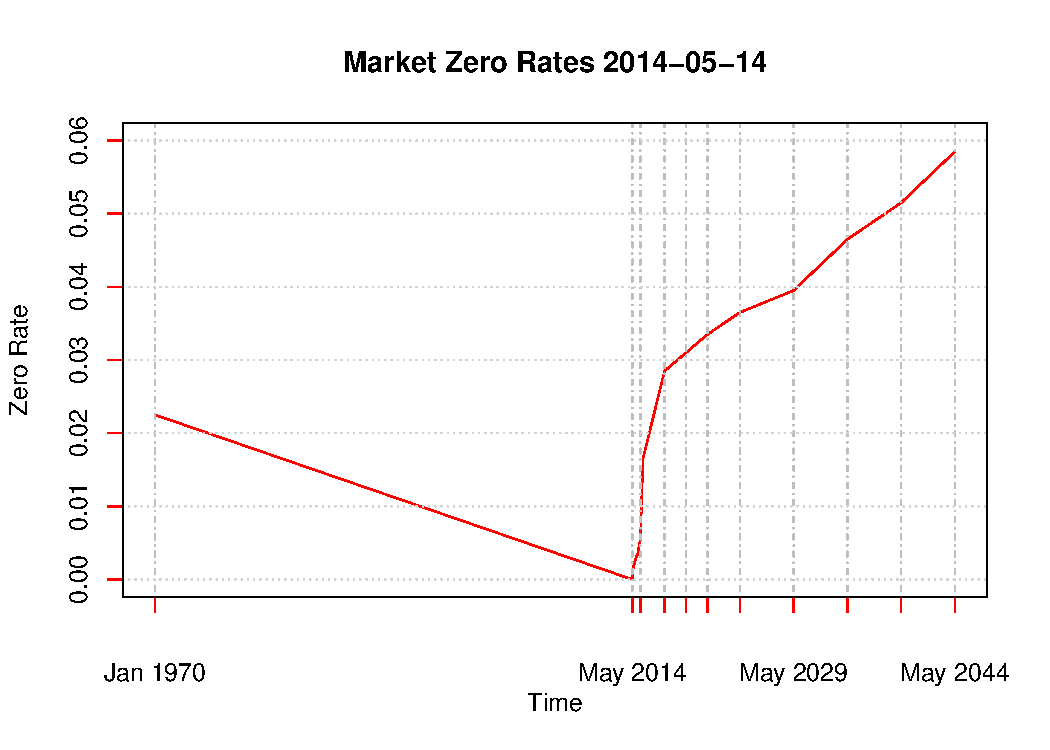
\includegraphics[width=\maxwidth]{figure/plot} 

\end{knitrout}


\end{document}
